\section{Terms, definitions and abbreviated terms}
\subsection{Terms and Definitions}
\begin{itemize}
    \item \textbf{OAuth}: Authentication protocol that allows one application 
    to interact with another one on behave of the first one.
    \item \textbf{Firebase Cloud Messaging}: Cross-platform message and 
    notification solution develop by Goodle.
    \item \textbf{Customer}: Type of user who is going to search and create 
    order by purchasing products from merchants
    \item \textbf{Merchant}: Store that upload products to the platform, from
    which the customers are going to purchase 
    \item \textbf{Driver}: User that fulfills the order generated by the 
    customer 
    \item \textbf{Order}: A list of items that was paid by the customer and 
    fulfilled by the driver.
    \item \textbf{Cart}: Container that temporary holds a group of products 
    that are going to be purchased.
    \item \textbf{Estimated time of Arrival}: The amount of time that 
    an order is going to take before arriving to the customer.
    \item \textbf{Interaction}: Amount of touches required by the user to 
    perform an action, if the device has a touch screen, or the amount of 
    clicks a user performs, if the device has a non-touch screen.
    \item \textbf{2FA}: Authentication methods in which a particular device is 
    used to grand access to a website or application, if two or more pieces of 
    evidence confirm the user identity.
\end{itemize}

\subsection{Abbreviated Terms}
\begin{itemize}
    \item \textbf{PSS}: Personal Shopper System
    \item \textbf{PSMS}: Personal Shopper Merchant System
    \item \textbf{PSDS}: Personal Shopper Driver System
    \item \textbf{PSSS}: Personal Shopper Server System
    \item \textbf{FCM}: Firebase Cloud Messaging
    \item \textbf{ETA}: Estimated time of Arrival
    \item \textbf{2FA}: 2-Factor Authentication
\end{itemize}

\pagebreak

\subsection{Assumptions and Dependencies}
\begin{enumerate}[label=AS-\arabic*]
    \item The drivers are already sign up in the system when they send their 
    driver application to the company
    \item The merchants are added into to the system outside of the 
    application scope
    \item The merchants are going to submit products that are appropriate for 
    all ages. \textit{They are not going to upload drugs, guns, 
    medical devices or sex toys}
    \item The merchants are already sign a contract that specify the types of 
    products they can add in the platform
    \item Customers do not have support for 2FA
    \item PSS, PSMS, PSDS only talk with PSSS, using a 
    request-response approach.
\end{enumerate}
\begin{figure}[!htb]
    \centering
    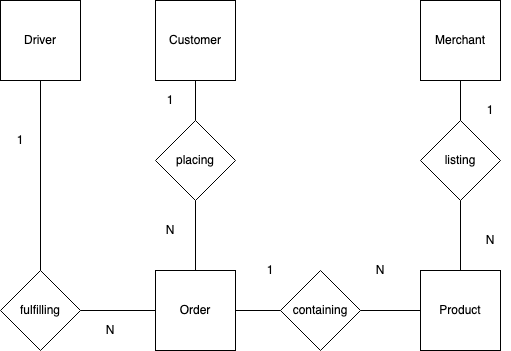
\includegraphics[scale=0.70]{Logical Data Model.png}
    \caption{Logical Data Model}
\end{figure}

\pagebreak

\begin{enumerate}[resume, label=AS-\arabic*]
    \item Merchants have no more than 5 employees
    \item All the merchants, costumers and drivers operate inside the 
    Hoboken area
    \item PSS have two versions mobile which is Android and a Web version
    \item PSMS has only a web version
    \item PSDS has only an Android version
    \item PSSS is an API server only
    \item Notifications in PSS (Mobile/Web) and PSDS are going to use FCM
\end{enumerate}

\pagebreak

\subsection{Operating Environment}
\begin{enumerate}[label=OE-\arabic*]
    \item The PSSS is going to run on AWS infrastructure
    \item Image assets are going to be stored in AWS S3
    \item New servers are going to be spin up on demand using EC2 VMS
    \item The PSSS can only be accessed by PSS, PSMS, PSDS 
    \item Network requests coming from outside of US are going to be ignored
\end{enumerate}
\begin{figure}[!htb]
    \centering
    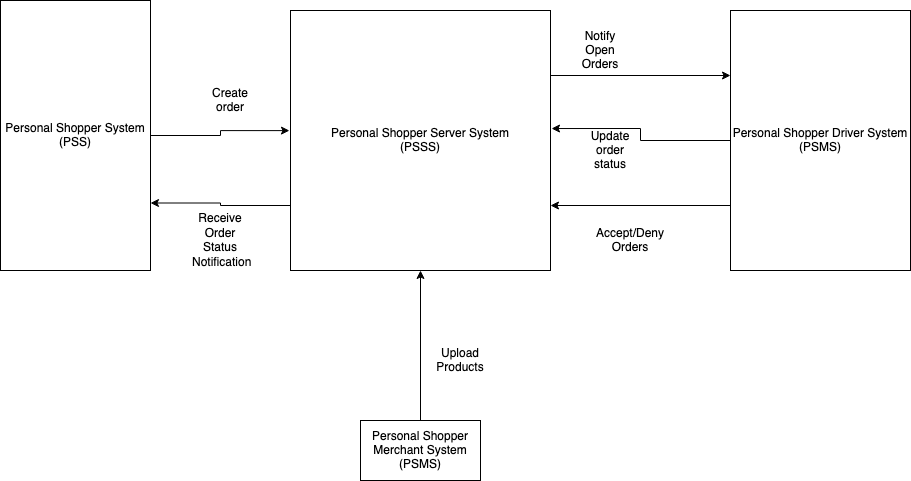
\includegraphics[scale=0.40]{Context Diagram.png}
    \caption{Context Diagram}
\end{figure}